\documentclass{article}
\usepackage{indentfirst}
\usepackage{lmodern}
\usepackage[utf8]{inputenc}
\usepackage[T1]{fontenc}
\usepackage[ngerman]{babel}
\usepackage{amssymb,amstext,amsmath}
\usepackage{graphicx}
\usepackage{dsfont}
\usepackage{amsfonts}
\usepackage{graphics}
\usepackage{float}
\usepackage{cite}
\usepackage{url}
\usepackage{capt-of}
%\pagestyle{empty}
\usepackage{floatflt}
\usepackage{tabularx}

 
\title{Wechelstromkreis}
\author{Alexander Heinisch, Dominik Wille}
\begin{document}
\maketitle
\vspace{13cm}
\noindent
\begin{center}
\begin{tabular}{r l}
Tutor & Sebastian Baum  \\
Durchführung & 15. Mai 2013 von 14:00 - 18:00 \\

E-Mail Dominik & dominik.wille@fu-berlin.de \\
E-Mail Alexander & Matthias.Heinisch@gmx.de \\
\end{tabular}
\end{center}

\newpage
\tableofcontents
\newpage


\section{Ziele des Versuchs}
In diesem Versuch untersuchen wir Widerstände, Kondensatoren, Spulen und deren Kombination, die Wechselstromkreise. Diese Beschreiben wir durch komplexe Widerstandsoperatoren und Ersatzschaltbilder
\section{Physikalische Grundlagen}
\subsection{Strom und Spannung an Widerständen, Kondensatoren und Induktivitäten}
In diesem Versuch sind die Schaltkreise aus den Bauelementen Kondensator, Spule und Widerstand mit den Messgrößen Kapazität \(C\), Induktivität \(L\) und Widerstand \(R\) zusammengesetzt. Sie werden durch folgende Zusammenhänge zwischen Strom I und Spannung U bestimmt:

\begin{equation}
\label{1}
Widerstand\ R: U_{R}=-R\cdot I_{R}
\end{equation}
\begin{equation}
\label{2}
Kapazität\ C: I_C=-C\frac{dU_C}{dt}
\end{equation}
\begin{equation}
\label{3}
Induktivität\ L: U_{L}=-L\frac{dI_{L}}{dt}
\end{equation}

dabei sind: \vspace{0,5cm}

\begin{tabular}{l l}
\(\ U_{R}\) & := Spannung am Widerstand\\
\(\ R\)		& := Widerstand\\
\(\ I_{R}\)	& := Strom am Widerstand\\
\(\ I_{C}\)	& := Strom am Kondensator\\
\(\ C\)		& := Kapazität des Kondensators\\
\(\ \frac{dU_{C}}{dt}\)	& := Änderung der Spannung am Kondensator mit der Zeit\\
\(\ U_{L}\)	& := Spannung an der Spule\\
\(\ L\)		& := Induktivität der Spule\\
\(\ \frac{dI_{L}}{dt}\)	& := Änderung des Stroms an der Spule mit der Zeit\\
\vspace{0,5cm}
\end{tabular}\\

Die Größen R, C und L sind positiv definiert. Allerdings setzt die Beziehung zwischen Spannung und Strom aufgrund der Kirchhoff'schen Regeln ein Minuszeichen voraus denn jeder Leiter besitzt einen Widerstand, woraus eine Gegenspannung resultiert. Im Falle des Kondensators bewirkt ein positiver Strom eine Erniedrigung der Spannung und in einer Spule wird eine Spannung induziert sobald sich der Strom ändert.

\subsection{Wechselspannung an Widerständen, Kondensatoren 
Induktivitäten und Impedanzen }
\subsubsection{Wechselstrom und Wechselspannung}
Eine Wechselspannung bzw. ein Wechselstrom hat eine charakteristische sinus- oder cosinusförmige Spannung bzw. Strömung. Sie werden wie folgt bezeichnet:

\begin{equation}
\label{4}
U_{t}=U_{0}\cdot cos(\omega t+\varphi _{1})\ \ bzw.\ \ I_{t}=I_{0}\cdot cos(\omega t+\varphi _{2})
\end{equation}

Häufig werden auch komplexe Größen verwendet, da sich hierdurch viele Gleichungen vereinfachen.

\begin{equation}
\label{komplex}
U_{t}=Re \left( U_{0}\cdot e^{i\left(\omega t+\varphi _{1}\right)}\right)\ \ bzw.\ \  I_{t}=Re \left(I_{0}\cdot e^{i\left(\omega t+\varphi _{2}\right)}\right)
\end{equation}

\begin{tabular}{l l}
\(\ I_{0}\)	&	:= Maximalstrom\\
\(\ U_{0}\) &	:= Maximalspannung\\
\(\ \omega\)&	:= Kreisfrequenz\\
\(\ \varphi\)&	:= verschiedene Phasen
\end{tabular}\\

Dabei treten in Schaltkreisen mit \(R\), \(C\) und \(L\) durch Wechselspannungen Wechselströme gleicher Frequenz und Phasenverschiebungen zwischen Strom und Spannung auf. Zum Vereinfachen setzt man daher die Phase der Spannung gleich Null \(\ (\varphi _{1}=0)\) \\

\subsubsection{Impedanz Z}
Die Impedanz \(Z\) (Wechselstromwiderstand) beschreibt das Verhältnis von der Spannungs- zur Stromamplitude.

\begin{equation}
\label{5}
Z=\frac{U_{0}}{I_{0}}
\end{equation}

Setzten wir nun die Gl.\(\ \eqref{4}\) in Gl.\(\ \eqref{1}\) bis \(\ \eqref{3}\) ein, so erhalten wir die Impedanzen der Bauteile und die Phasenverschiebung des Stroms zur Spannung an R, C und L:

\begin{equation}
Z_{R}=R
\end{equation}
\begin{equation}
\varphi = \pi
\end{equation}

Für die Kondensatoren gilt des weiteren:

\begin{equation}
Z_{C}=\frac{1}{i \omega C} = \frac{-i}{\omega C}
\end{equation}
\begin{equation}
\varphi=\frac{-\pi }{2}
\end{equation}

Der Strom eilt hier der Spannung voraus. Außerdem gilt für Spulen:

\begin{equation}
Z_{L}= i \omega L\ \ und \ \ \varphi =+\frac{\pi }{2}
\end{equation}

wobei hier der Strom der Spannung hinterher läuft.

\subsubsection{Wechselstromnetzwerke}
Hier gelten die gleichen Regeln wie beim Gleichstromfall, nur dass hierfür die komplexe Impedanz benutzt wird.
Für die Reihenschaltung gilt:
\begin{equation}
Z=\mid{ \sum \limits_{i} Z_i} \mid
\end{equation}
\begin{equation}
tan \varphi ={\frac{Im \left( \sum \limits_{i} Z_{i} \right) }{Re \left( \sum \limits_{i} Z_{i} \right) }}
\end{equation}
und für die Parallelschaltung:

\begin{equation}
\frac{1}{Z}=\mid{ \sum \limits_{i} \frac{1}{Z_{i}}}\mid 
\end{equation}
\begin{equation}
tan\varphi = {\frac{Im \left( {\sum\limits_{i}{\frac{1}{Z_i}}} \right) }{Re \left( {\sum\limits_{i}{\frac{1}{Z_i}}}\right) }}
\end{equation}

\subsection{Wechselstromleistung}
Die Wechselstromleistung ergibt sich aus dem Produkt der Realteile von U und I:

\begin{equation}
P=Re(U)\cdot Re(I)=\frac{1}{2}(U+U^*)\cdot \frac{1}{2}(I+I^*)
\end{equation}
Wenn wir Wechselströme komplex darstellen, ergibt sich:

\begin{equation}
U(t)_{komplex}=U_{0}e^{i\omega t}
\end{equation}
\begin{equation}
I(t)_{komplex}=I_{0}e^{i\omega t+\varphi}
\end{equation}
Für das zeitliche Mittel folgt daraus:

\begin{equation}
\overline{P}=\frac{1}{4}\left[U_{0}I_{0}(e^{i\varphi }+e^{-i\varphi })\right]
\end{equation}

Nun führen wir die Effektivwerte für Spannung und Strom ein mit:
\begin{equation}
U_{eff}=\frac{U_{0}}{\sqrt{2}}
\end{equation}
\begin{equation}
I_{eff}=\frac{I_{0}}{\sqrt{2}}
\end{equation}

Und daraus folgt nun für die Leistung P:
\begin{equation}
P=U_{eff}I_{eff}cos \varphi
\end{equation}

\subsection{Leistungsverluste}
Ideale Spulen und Kondensatoren arbeiten verlustfrei, in realen Spulen hingegen entzieht unter anderem der Widerstand des Drahtes dem System Energie. Auch Wirbelstromverluste in leitenden Materialien und Ummagnetisierungsverluste bei Spulen mit Eisen- oder Ferrimagneten entziehen dem System Energie.
Der Verlustfaktor d beschreibt das Verhältnis des Verlustwiderstandes zum rein kapazitiven oder induktiven Widerstand:

\begin{equation}
d=\frac{1}{tan \varphi }
\end{equation}

\subsection{Ersatzschaltbilder}
Um die Verluste an realen Spulen zu beschreiben, benutzt man als Ersatzschaltbild die Serienschaltung von einer Spule und einem Widerstand.
\begin{center}
\begin{minipage}{\linewidth}
\centering
\makebox[0cm]{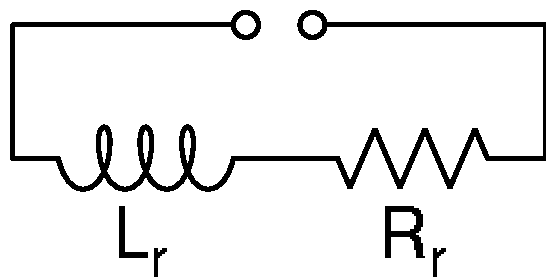
\includegraphics[width=3cm]{ersatz}}
\captionof{figure}{Ersatzschaltbild Serienschaltung}
\end{minipage}
\end{center}
\begin{align}
Z&= R+wL_r\\
|Z|&=\sqrt{R_{r}^2+(\omega L_{r})^2}\\
tan \varphi &=-\frac{\omega L_{r}}{R_{r}}
\end{align}
Analog verwendet man bei einer Parallelschaltung \((R_{p}\ und\ L_{p}) \):
\begin{center}
\begin{minipage}{\linewidth}
\centering
\makebox[0cm]{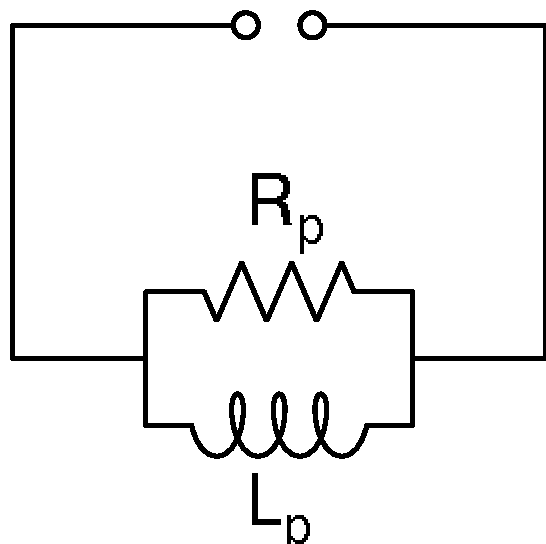
\includegraphics[width=3cm]{ersatz2}}
\captionof{figure}{Ersatzschaltbild Parallelschaltung}
\end{minipage}
\end{center}
\begin{equation}
\frac{1}{Z}=\sqrt{\frac{1}{R_{p}^2}+\frac{1}{(\omega L_{p})^2}}
\end{equation}
\begin{equation}
tan\varphi =-\frac{R_{p}}{\omega L_{p}}
\end{equation}
\subsection{Filter (Hoch-, Band-, Tiefpass)}
Die Kombinationen von R-C-L-Gliedern stellen Spannungsteiler dar.
Ein R-C-L-Bandpass ist ein schwingungsfähiges System, welches ein Impedanzminimum bei Resonanz eines Siebkreises, bzw. ein Maximum bei einem Sperrkreis aufweist.

\subsection{Wechselstrombrücke}
Eine Wechselstrombrücke (Wheatstonesche Brücke) ermöglicht die Messung von Induktivität und Kapazität, wenn die Impedanz übereinstimmt.\\
Es gilt:
\begin{equation}
\frac{L_{x}}{L_{0}}=\frac{R_{a}}{R_{b}}
\end{equation}
\begin{equation}
\frac{R_{x}+R'}{R}=\frac{R_{a}}{R_{b}}
\end{equation}
Mit dem Phasenabgleichswiderstand \(R'\) wird bei dem Bauteil die Phase verschoben.

\newpage
\section{Aufgabenstellung}
\subsection*{Aufgabe 1}
Aufbau eines R-C-Kreises. Einstellung der charakteristischen Frequenz mit \(\ U_{R}=U_{C} \). Messung der Generator- und der Teilspannung und Bestimmung der Phasenverschiebung. Unabhängige Messung von R und C mit einem Multimeter und Vergleich der Beobachtung am R-C-Kreis mit den theoretischen Erwartungen. 

\subsection*{Aufgabe 2}
Messung des Frequenzbereichs \(\frac{U_{R}}{U_{G}}\)\ (Verbraucherspannung zu Generatorspannung) an einer Tonfrequenzweiche (Drei-Wege-Weiche mit R-L-Weiche mit R-L-Tiefpass, R-C-L-Bandpass und R-C-Hochpass) und Vergleich mit dem theoretischen Verlauf durch unabhängige Messung der Werte der Widerstände, Kapazitäten und Induktivitäten mit Digital-Multimeter

\subsection*{Aufgabe 3}
Messung der Induktivität und des Verlustwiderstandes einer der beiden Spulen aus Aufgabe 2 mit einer Wechselstrombrücke und Vergleich mit der unabhängigen Messung (Digitalmultimeter) von L und dem Gleichstromwiderstände R der Spule.

\newpage

%\section{Auswertung}
\section{Aufgabe 1}
\begin{center}
\begin{minipage}{\linewidth}
\centering
\makebox[0cm]{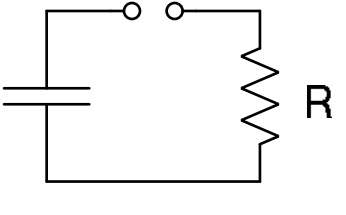
\includegraphics[scale=0.5]{sb1}}
\captionof{figure}{Schaltplan Aufgabe 1}%
\label{schaltplan_nr1}
\end{minipage}
\end{center}

Für diese Aufgabe haben wir einen Kondensator mit einem Widerstand in Reihe geschalten (siehe Abbildung 1.1). Mit einem Frequenzgenerator legten wir eine Spannung an und mit Hilfe eines Oszilloskops veränderten wir die Frequenz, bis beide Sinuskurven die gleiche Spannung hatten. 
Damit die Teilspannung an der Spule und am Kondensator übereinstimmen muss folgendes gelten:
\begin{equation}
U_C = U_R 	\Rightarrow	 U_{ges} = U_C + U_R
\end{equation}
Mit einem Spannungsmessgerät (Fluke 175) haben wir die Spannung zwischen dem Widerstand und dem Kondensator gemessen. Dabei betrug der Spannungsunterschied:
\begin{equation}
\notag
\Delta U=0,023 V
\end{equation}

Die Frequenz betrug dabei konstant:

\begin{equation}\notag
f_{char} = (160,45\pm 0,1) Hz
\end{equation}

Die verwendeten Bauteile des R-C-Kreises wurden separat noch einmal nachgemessen, dabei ergab sich für den Widerstand einen Wert von:
\begin{equation}\notag
R = (0.990 \pm 0.012)k\Omega
\end{equation}

und die Kapazität des Kondensators:
\begin{equation}\notag
C = (1.001 \pm 0.013)\mu F
\end{equation}

Die Fehler errechnen sich aus $\pm (1.0\% +3dgt)$.

\subsection{Berechnung der Frequenz}
Nun können wir über folgende Formel den theoretischen Wert der Frequenz f berechnen:
\begin{equation}\notag
f_{theo}=\frac{1}{2\pi RC}= (160.6 \pm 2.0)Hz
\end{equation}

Den Fehler bestimmen wir über die Gauß'sche Fehlerfortpflanzung:
\begin{equation}\notag
\Delta f_{theo}=\sqrt{\left(\frac{\partial f_{theo}}{\partial R}\cdot \Delta R\right)^2+\left(\frac{\partial f_{theo}}{\partial C}\cdot \Delta C\right)^2}
\end{equation}

\subsection{Phasenverschiebung}
Für die Phasenverschiebung haben wir bei einer Frequenz von f = 160,30 HZ am Oszilloskop ein \(\Delta\)t = 0,8ms abgelesen. Dafür ergibt sich für \(\phi\) einen Wert für:
\begin{equation}
\notag
\phi = 2\pi f \Delta t = (0,806 \pm 0,009)^\circ = (0,257\pm 0,003)\pi
\end{equation}

Somit ergibt sich wie erwartet \(\frac{\pi}{4}\) für die Phasenverschiebung.
Um nun noch die Phasenverschiebung auszurechnen, benutzten wir:
\begin{equation}\notag
\phi_{theo}=arctan\left(\frac{1}{\omega RC}\right)=\left(0,7854 \pm 0.0065\right)^\circ =(0,250\pm 0,003)\pi
\end{equation}

Den Fehler bekommen wir aus:
\begin{equation}\notag
\Delta \phi_{theo}=\sqrt{\left(\frac{\partial \phi_{theo}}{\partial f_{theo}}\cdot \Delta f_{theo}\right)^2+\left(\frac{\partial \phi_{theo}}{\partial C}\cdot \Delta C\right)^2+\left(\frac{\partial \phi_{theo}}{\partial R}\cdot \Delta R\right)^2}
\end{equation}

\subsection*{Fazit}
Den Wert für die charakteristische Frequenz konnten wir relativ schnell finden, nachdem wir festgestellt hatten, dass ein Messgerät einen Wackelkontakt hatte und bis dahin nur seltsame Werte geliefert wurden.\\
Der theoretische und der gemessene Wert der charakteristische Frequenz sind gleich, nur dass der Fehler des theoretischen Werts aufgrund der Bauteile doch relativ groß ist. Die Phasenverschiebung ist auch ziemlich klein.
\newpage
\section{Aufgabe 2}
\subsection{Abschätzung des Arbeitswiderstandes}

Um den Arbeitswiderstand zu bestimmen, benutzen wir das Vier-Quadranten-Kennlinienfeld (Abbildung 7) und gehen vom äußersten Punkt des dritten Quadranten für \(I_B\)= 140,8\(\mu A\) senkrecht nach oben. Im Zweiten Quadranten treffen wir so den Wert für \(I_C\)=13,9 mA, welches unser Startpunkt der Arbeitsgeraden (bzw. Kollektor-Widerstandsgerade) sein wird. Damit ergeben sich die Koordinaten (\(U_{CE}\) = 0[V], \(I_{C}\) = 13,9[mA]) für den Punkt \(P_1\) des Kurzschlussfalls. Der Punkt \(P_2\) liegt bei den Koordinaten (\(I_{C}\) = 0 [mA],\(U_{CE}\) = 12[V]), weil 12[V] die maximale Versorgungsspannung betrug.\\
Der Arbeitspunkt \(P_{A}\) liegt laut Definition bei \(\left(\frac{U_{CE}}{2}, \frac{I_{C}}{2}\right)\), welches bei uns den Werten (6.055[V],6.95[mA]) entspricht.\\

Den Arbeitswiderstand wird über die Formel:
\begin{equation}
\notag
R_{A}=\mid \frac{1}{m}\mid = \left(\frac{U_{EC}}{I_C}\right) = 871.23 \Omega
\end{equation}\\

Während des Versuchs haben wir für den Arbeitswiderstand einen Wert von (\(464.3\pm 2.6)\Omega\) gemessen.\\

Der Basisvorwiderstand ergibt sich aus der Formel:
\begin{equation}
\notag
R_V= \frac{U_{EC}-U_{EB}}{I_B}=\frac{6V-0.7V}{(63.5\cdot 10^{-6})A}=83.5k\Omega
\end{equation}

Hier hatten wir einen Wert von (\(100.2\pm 0.8)k\Omega\) gemessen. Auf die Unterschiede dieser Werte werden wir später in der Diskussion eingehen.

\subsection{Überprüfung der Kollektor-Widerstandsgeraden}

Nun überprüfen wir die abgeschätzten Werte, indem wir einen Arbeitswiderstand und einen Basisvorwiderstand in die Schaltung einbauen (siehe Abbildung 6) und eine neue Messreihe aufnehmen. Wir steigern dabei die Werte für \(I_B\) in gleichen Abständen und notieren, wie sich die anderen Größen dazu verhalten. \(U_0\) hielten wir konstant auf (\(12.11\pm 0.09\))

\newpage
Unsere Messung ergaben folgende Werte:\\

\begin{center}
\begin{tabular}{r r r r}
\(I_B [\mu A]\) & \(I_C [mA]\) & \(U_B [V]\) & \(U_{CE}[V]\) \\
\hline
\(52.116\) & \(9.0\) & \(0.116\) & \(7.93\) \\ 
\(62.519\) & \(9.3\) & \(0.191\) & \(7.75\) \\ 
\(72.518\) & \(9.7\) & \(0.255\) & \(7.59\) \\ 
\(81.305\) & \(10.0\) & \(0.315\) & \(7.45\) \\ 
\(94.132\) & \(10.5\) & \(0.362\) & \(7.22\) \\ 
\(101.505\) & \(10.9\) & \(0.429\) & \(7.01\) \\ 
\(113.423\) & \(11.8\) & \(0.526\) & \(6.61\) \\ 
\(122.311\) & \(12.6\) & \(0.586\) & \(6.24\) \\ 
\(131.906\) & \(22.7\) & \(0.755\) & \(1.52\) \\ 
\(142.410\) & \(23.4\) & \(0.757\) & \(1.17\)
\end{tabular}
\captionof{table}{Rohmesswerte für Aufgabe 2.2}
\end{center}

\newpage
\section{Aufgabe 3}
In dieser Aufgabe wurde eine Wechselstrombrücke aufgebaut um sowohl die Induktivität \(L_x\) als auch den Ohmschen Widerstand \(R_x\) der Spule vom Tiefpass aus Aufgabe 2 zu bestimmen. 

\subsection{Aufbau}
Hierfür wurde eine Schaltung auf dem Steckbrett nach folgendem Schaltplan aufgebaut. Die Phase zwischen den beiden Spannungsmesspunkten wurde mit dem Oszilloskop mit der ,,elliptischen Auftragung'' auf \(\varphi = 0 \) eigestellt. Und anschließend die Effektivspannung mit dem Fluke 175 gemessen
\begin{center}
\begin{minipage}{\linewidth}
\centering
\makebox[0cm]{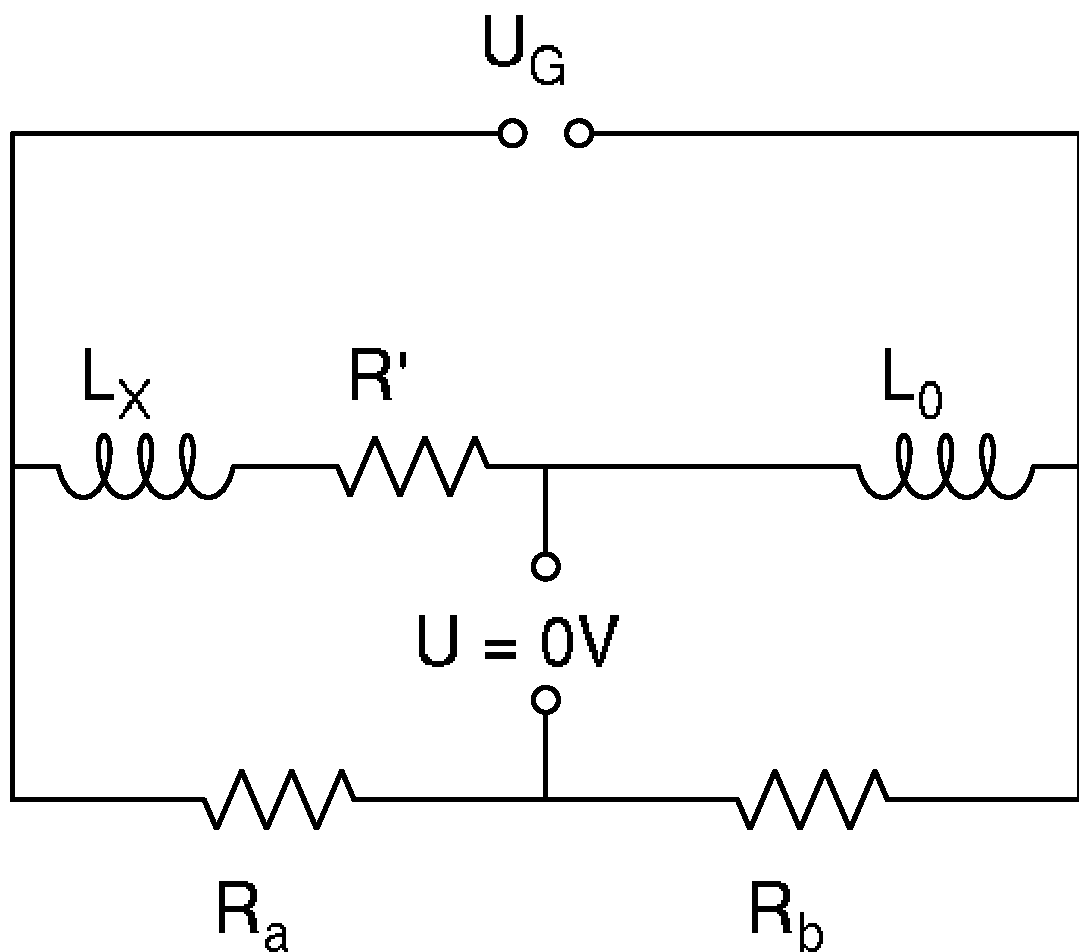
\includegraphics[width=6cm]{bruecke}}
\captionof{figure}{Schaltplan der Wechselstrombrücke}
\end{minipage}
\end{center}

\subsection{Gegebenes und Messwerte}
Separat wurden folgende Größen gemessen oder von den Aufschriften der Bauteile entnommen. Leider wurde vergessen zu notieren mit welchem Messgerät die Widerstände gemessen wurden die Fehler werden mit \(\Delta R = 1\% + 5d\) abgeschätzt.
\begin{center}
\begin{tabular}{c|c}
Messgröße & Messwert\\\hline
\(f\) & \((1999 \pm 14)\, Hz \) \\
\(L_0\) & \((1,507 \pm 0,020)\, mH \) \\
\(R_0\) & \((2,91 \pm 0,02)\, \Omega \) \\
\(R_a\) & \((761 \pm 13)\, \Omega \) \\
\(R_b\) & \((241,8 \pm 2,9)\, \Omega \) \\
\(R'\) & \((5,3 \pm 0,5)\, \Omega \) \\
\(f\) & \((1999 \pm 14)\, Hz \) \\ \hline
\(R_x\) & \(\left(3,7 \pm 0,5 \right)\, \Omega \) \\
\(L_x\) & \((4,82\pm 0,07)\, mH \) \\
\end{tabular}
\captionof{table}{Sepperate Messung aller Größen}%
\end{center}

\subsection{Auswertung}
Um nun aus den Vorhanden Messdaten \(L_x\) und \(R_x\) zu bestimmen, wird folgender Ansatz gemacht:
\begin{align}
\frac{Z_a}{Z_b} &= \frac{i\omega L_x + R'+ R_x}{i\omega L_0 + R_0}
\end{align}
Da über den Phasenabgleichswiderstand die Phase auf \(\varphi = 0\) gebracht wurde müssen die beiden Phasenverschiebungen der Spulen und Widerständen identisch sein. Daher gilt:
\begin{align}
\Rightarrow \frac{i\omega L_0}{R_0} &= \frac{i\omega L_x}{R'+R_x}\notag \\
\Rightarrow L_x &= \frac{L_0}{R_0}\cdot\left( R' + R_x \right) \label{L_x}
\end{align}
Außerdem wurden \(R_a\) und \(R_b\) derart gewählt, dass gelten muss:
\begin{align}
\frac{R_a}{R_b} &= \frac{\omega L_x + R' + R_x}{\omega L_0 + R_0}
\end{align}
Nach einsetzten von \eqref{L_x} formt sich das zu
\begin{equation}
R_x = \frac{R_a}{R_b} \cdot R_0 - R'
\end{equation} um.
Für die Fehler gilt nach Gaußscher Fehlerfortpflanzung:
\begin{align}
\Delta R_x &= \sqrt{
\left( \frac{R_0}{R_b} \cdot \Delta R_a \right)^2 +
\left( \frac{R_a}{R_b} \cdot \Delta R_0 \right)^2 +
\left( \frac{R_a}{R_b^2} \cdot \Delta R_b \right)^2 +
\left( \Delta R' \right)^2
}\notag \\
\Delta L_x &= \sqrt{
\left( \frac{R'+R_x}{R_0} \Delta L_0 \right)^2 +
\left( \frac{L_0\left( R'+R_x \right)}{R_0^2}  \cdot \Delta R_0 \right)^2 +
\left( \frac{L_0}{R_0} \cdot \Delta R' \right)^2 +
\left( \frac{L_0}{R_0} \cdot \Delta R_x \right)^2
}\notag
\end{align}
Ausgerechnet ergibt das:
\begin{center}
\begin{tabular}{c|c}
Messgröße & Errechneter Wert\\\hline
\(R_x\) & \(\left(3,86 \pm 0,23 \right)\, \Omega \) \\
\(L_x\) & \((4,74\pm 0,50)\, mH \) \\
\end{tabular}
\captionof{table}{Mit der Apparatur ermittelte Größen}
\end{center}

\subsection{Fazit}
Die ermittelten werte für die Induktivität und den ohmschen Widerstand der Spule sind identisch zu den direkt mit dem Messgerät gemessenen Werten. dabei konnte sogar die Genauigkeit der Widerstandsmessung der Spule erhöht werden, da diese sonst nur mit dem für kleine Widerstände sehr ungenauem VC230 oder Fluke 175 gemessen werden konnten.
\begin{center}
\begin{tabular}{c|c|c}
Messgröße & Errechneter Wert & Vergleichswert\\\hline
\(R_x\) & \(\left(3,9 \pm 0,3 \right)\, \Omega \) &  \(\left(3,7 \pm 0,5 \right)\, \Omega \)\\
\(L_x\) & \((4,7\pm 1,7)\, mH \) & \((4,82\pm 0,07)\, mH\) \\
\end{tabular}
\captionof{table}{Mit der Apparatur ermittelte Größen}
\end{center}

\section{Fazit}
Alle drei Aufgaben waren sehr gut durchführbar. Alle Geräte haben durchgehend funktioniert und waren leicht zu bedienen. Besonders das moderne Oszilloskop sorgte für vergleichsweise gute Messdaten. Die Ergebnisse waren zufriedenstellend und wir können die Versuche zu den Wechselstromkreisen auf jeden Fall zu den angenehmen und gleichzeitig interessanten Versuchen zählen.

\section{Qellenangabe}
\begin{itemize}
\item GPII-Skript
\item Platzskript
\item Die Graphen wurden mit GNU-Plot erstellt
\item Die Schaltpläne wurden mit XCircuit erstellt
\end{itemize}
\vspace{7.0cm}

\begin{tabularx}{\textwidth}[b]{p{5cm} X p{5cm}} \cline{1-1} \cline{3-3}
Datum, Dominik Wille & & Datum, Alexander Heinisch
\end{tabularx}
\end{document}